\begin{frame}
    \frametitle{GPU Computing}
    \framesubtitle{Introduction}
    \begin{itemize}
        \item At the beggining, programming in GPU was really difficult.
        \item Now, there are a lot of languages, applications, libraries, etc
            who really help to enter in the GPU Computing world.
        \begin{itemize}
            \item OpenCL, CUDA.
            \item MATLAB.
            \item CUBLAS, CUSP, Thrust, etc.
        \end{itemize}
    \end{itemize}
\end{frame}

\begin{frame}
    \frametitle{GPU Computing}
    \framesubtitle{Architecture}
    \begin{figure}
        \centering
        \label{fig:architecture}
        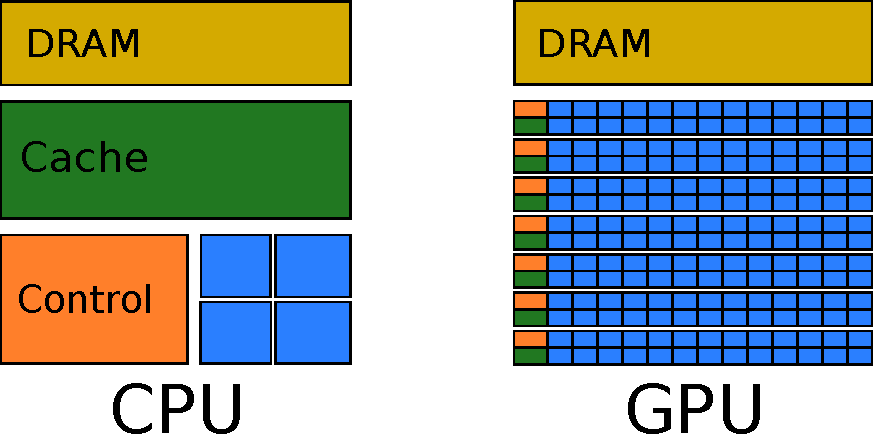
\includegraphics[width=0.8\textwidth]{img/architecture.pdf}
        \caption{CPU and GPU simplistic architecture model}
    \end{figure}
\end{frame}

\begin{frame}
    \frametitle{GPU Computing}
    \framesubtitle{Differences between CPU and GPU}
    \begin{itemize}
        \item Goals and design
        \begin{itemize}
            \item The CPU was designed to have a good performances with parallel and non-parallel
                  scenarios.
            \item The GPU was dessigned to do highly parallel work.
        \end{itemize}
        \item The CPU minimize \blue{latency} experienced by 1 thread (big on-chip caches).
        \item The GPU maximize \blue{throughput} of all threads.
    \end{itemize}
\end{frame}
